\documentclass{article}
\usepackage{graphicx} % Required for inserting images

\title{Chip-Firing Games}
\author{Eric Yee}
\date{June 2023}

\begin{document}

\maketitle
Have you ever been at the beach and with a handful of sand, start sprinkling the tiny grains such that it begins to form this perfect cone of sand? But while you're admiring this beautifully symmetric creation, a process of destruction inevitably begins to take place. Starting with a single grain of sand beginning to slip, it will crash into multiple other grains causing it also to slip, and you can only watch in horror as one grain after another cascades into each other and an entire face of your beautiful sand cone collapses! \\

\begin{center}
    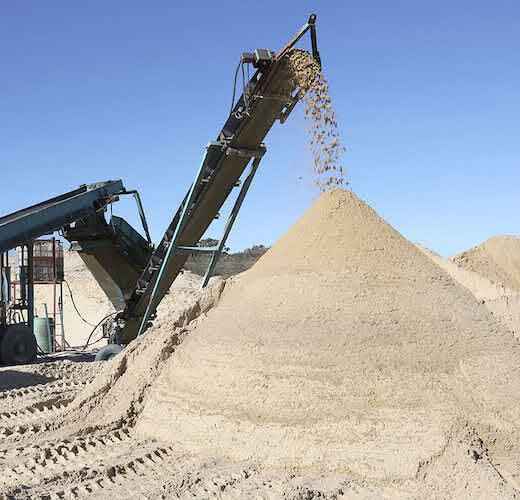
\includegraphics[width=10cm, scale=1.5]{Magazines/sept23/images/sand.jpg}
\end{center}

However, to many of us, that dramatic avalanche of sand might not only trigger grief, but also a primal longing to model this network of sand in which, individual stacks of sand are able to send sand to adjacent stacks, leading to these destructive avalanches.\\

Well if that is you, look no further, because we will now find such a model once and for all!\\

First, we need to decide what our network will be, and how we will represent sand. Our best choice for the network is the tried and true connected graph $G(V,E)$ where two vertices are adjacent if they share an edge. Thus we can drop individual grains of sand at each vertex, and we will call each of these grains "chips", such that the chip configuration of our graph will be $\{c_1,c_2,...,c_n\}$ where $c_i$ is the number of chips/sand at vertex $v_i$.\\

Now to replicate the avalanches we saw on the beach, we also define a vertex to "fire" as sending $1$ of its chips to each adjacent vertex. This way we hope that if enough vertices fire simultaneously we will see the entire sand pile collapse. Wait! But what if a vertex has fewer chips than adjacent vertices, after all, we can't have a stack of sand with negative sand! So we will call a vertex $v_i$ "ready to fire" iff the vertex has more chips than adjacent vertecies (ie. $c_i>\deg{v_i}$), and our model will consist of choosing a vertex that is "ready to fire", firing it, then repeating.\\

This all seems great, we have created our model and can watch these avalanches without going to the beach, yet it seems slightly uncomfortable that we must \emph{choose} a vertex to fire among those "ready to fire"... I mean we can't have freedom of choice in math! But does it actually make a difference which one you choose to fire first? Let's see what happens if we fire one vertex instead of another.\\

Let's say $v_1$ and $v_2$ are both ready to fire, and we decide to fire $v_1$ first. We see that firing $v_1$ could only have increased the chips at $v_2$, so $v_2$ is still able to fire! In this way, since any vertex that is ready to fire will always be ready to fire until it is actually fired, the way we select what to fire doesn't actually matter. Aha! Once again we see that free choice is just an illusion!\\

Now let's have some fun playing out this game with some different initial configurations. 

\begin{center}
    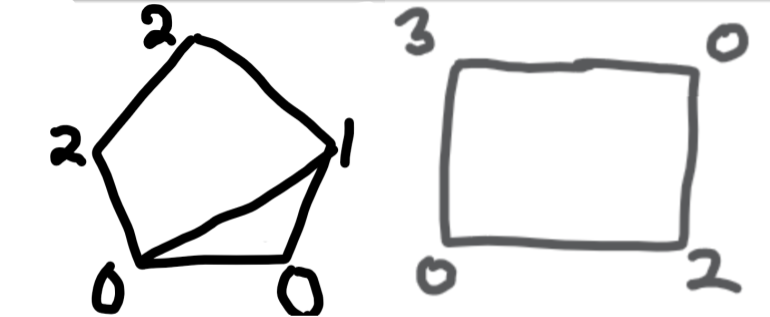
\includegraphics[width=10cm, scale=1]{images/example configs.png}
\end{center}

Hmmm... Sometimes our model seems to reach a chip configuration where no chip is "ready to fire", but other times it seems to go on forever. We'll call a chip configuration in which no vertex can fire as "stable", and these will mark the end of our game. \\

Now this seems to give rise to the question: which configurations will end in a stable configuration and which will go on forever? \\

To answer this, we'll look at the total number of chips. If the number of total chips $c$ in the system is greater than $2m-n$, where $n$ is the number of vertices and $m$ is the number of edges, then since $$\sum \deg{v_i}=2m,$$ by pigeon-hole principle one vertex will always have at least $\deg{v_i}$ chips. Thus there will always be a vertex "ready to fire" and our sand will move around forever.\\

Now let's attempt a lower bound: What if $c$ is less than $m$? Let's say we have a number of all the chips/sand grains prior to firing, this way they are distinct. If we begin firing vertices, we can assign each chip to the edge it first travels down. This way we can imagine that every time a vertex fires, chips just travels across the edge it was assigned, so that ways each chip is always on one of the endpoints of its assigned edge. But because $c<m$, there will always be at least one edge without a chip assigned to it, which means both vertices that are the endpoints of that edge will never fire. And moreover, in a connected graph that fires forever, a vertex that never fires will always be taking up chips from its surrounding vertices, making it impossible for the graph to fire forever! \\
\end{document}

what you have always longed for is, in fact, a concept called the chip-firing games. These 1-player games occur on a connected undirected graph where each vertex is given a certain number of chips (or, in our case, sand). The basic rules are:
\begin{enumerate}
    \item Let $c=\{c_1,c_2,...,c_n\}$ be the chip configuration, where $c_i$ is the number of chips at $v_i$, and $c_i$ is a positive integer.
    \item The vertex $v_i$ is "ready to fire" if $c_i\geq \deg{v_i}.$
    \item When a vertex fires, it sends one of its chips to each of the adjacent vertices.
    \item The process of the game is selecting a vertex that is "ready to fire," firing it, then repeating. If you reach a chip configuration where no vertex is "ready to fire," then the game ends, and you have reached a "stable configuration."
\end{enumerate}

Yet it seems uncomfortable that we need to randomly choose a vertex to fire among those "ready to fire". So let's see what happens if we fire one vertex instead of another.

Let's say $v_1$ and $v_2$ are both ready to fire, and we decide to fire $v_1$ first. We see that firing $v_1$ could only have increased the chips at $v_2$, so $v_2$ is still able to fire! In this way, since any vertex that is ready to fire, will always be ready to fire until it is actually fired, the way we select what to fire doesn't actually matter!

Since the order doesn't matter we also know that there is only one distinct set of firings that creates